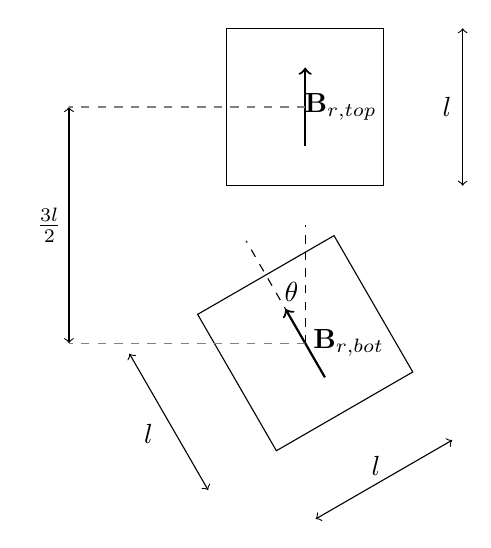
\begin{tikzpicture}

% Set up coordinates of vertices
\coordinate(toptl) at (-1,4);
\coordinate(toptr) at (1,4);
\coordinate(topbl) at (-1,2);
\coordinate(topbr) at (1,2);
\coordinate(bottl) at (0.366,1.366);
\coordinate(bottr) at (-1.366,0.366);
\coordinate(botbl) at (1.366,-0.366);
\coordinate(botbr) at (-0.366,-1.366);

% Draw magnets
\draw (toptl) -- (toptr) -- (topbr) -- (topbl) -- cycle;
\draw (bottl) -- (bottr) -- (botbr) -- (botbl) -- cycle;

% Draw magnetisation vectors
\draw[->,thick] (0,2.5) -- (0,3.5);
\draw[->,thick] (0.25,-0.433) -- (-0.25,0.433);
\node(Mtop) at (0.45,3) {\(\mathbf{B}_{r\text{,top}}\)};
\node(Mbot) at (0.55,-0) {\(\mathbf{B}_{r\text{,bot}}\)};

% Draw centres
%\node(ctop) at (0,4) {\textbf{.}};
%\node(cbot) at (0,0) {\textbf{.}};

% Draw dimensions
\draw[<->] (2,2) -- (2,4);
\node(lsidetop) at (1.8,3) {\(l\)};
\draw[<->] (-2.232,-0.134) -- (-1.232,-1.866);
\node(lsidebot) at (-1.99,-1.15) {\(l\)};
\draw[<->] (1.866,-1.232) -- (0.134,-2.232);
\node(lunder) at (0.9,-1.559) {\(l\)};
\draw[<->] (-3,0) -- (-3,3);
\node(d) at (-3.25,1.5) {\(\frac{3l}{2}\)};

% Draw horizontal centrelines
\draw[dashed,gray] (0,3) -- (-3,3);
\draw[dashed,gray] (0,0) -- (-3,0);

% Draw angle
\draw[dashed] (0,0) -- (0,1.5);
\draw[dashed] (0,0) -- (-0.75,1.3);
\node(theta) at (-0.175,0.65) {\(\theta\)};

\end{tikzpicture}